\section*{Appendix}
\widowpenalty=10000\clubpenalty=10000
\addcontentsline{toc}{section}{Appendix}
\renewcommand{\thesubsection}{\Alph{subsection}}\setcounter{subsection}{0}

\subsection{Implementation and training details}
\label{app:details}
\textbf{Prediction horizons and coordinates.}
The current model predicts 32 action steps in an 80-dimensional typed layout. Consequences use 16
steps with 48 available keypoint slots, each containing two displacement coordinates and one
observability coordinate. The agent sequence therefore contains 49 tokens: one state token, 32
action tokens, and 16 consequence tokens. Slots are shared storage positions with source-specific
validity masks. The current LIBERO adapter fills 39 consequence slots; EgoDex fills 14 hand-point
slots. Unused slots carry a false mask.

Actions use source adapters that preserve the physical meaning of pose, aperture, and joint
coordinates. Rotation is represented by the first two columns of its rotation matrix, concatenated
in column order, and bypasses statistical scaling. Gripper aperture is first expressed from closed
to open in the interval $[0,1]$ and then mapped to $[-1,1]$. The active robot recipe uses per-source
first and ninety-ninth percentiles for the remaining valid coordinates, with clipping to $[-1,1]$.
Min--max and standard-score normalization are supported alternatives; the archived runs identify the
active choice. Displacement uses image-normalized coordinates with gain 4. Observability remains a
separate target, including for occluded points whose displacement is masked.

\textbf{Temporal and visual inputs.}
A window selects nine frames at a stride of four source steps, spanning 33 time indices. The video
autoencoder produces a clean observation latent followed by future latents. The image canvas is
$384\times256$ pixels for the two-view template and $384\times320$ for the three-view template. The
template reserves positions for unavailable views rather than inventing additional observations.
DROID and Bridge are sampled at 15 and 5 Hz. The EgoDex training export retains every third
frame of the original 30 Hz stream, giving 10 Hz. This corrects the earlier 30 Hz description.
The RoboMIND sources lack native timestamps in the inspected export; their duration audit retains
a 15--20 Hz range rather than asserting a single measured rate.
Consequently, a step horizon corresponds to different elapsed durations across sources.
Duration-matched comparisons are a separate control for cross-source transfer.

\textbf{Noise sampling and weighting.}
For a uniform random variable $u$ and shift $r$, the implemented level is $\tau=ru/(1+(r-1)u)$. The
world and action shifts are 5 in the archived runs; the independent consequence draw uses the action
shift. The bell-shaped weight is proportional to $\exp[-2(\tau-1/2)^2]-\exp(-1/2)$, normalized by
its mean under the shifted sampling distribution. World, action, and consequence levels are
independent during training. The default sampling path decreases all three levels together with 10
Euler steps. Current training uses no additional probability mass on clamped boundary conditions. A
boundary-mixture comparison is planned independently of the primary coupling comparison.

\textbf{Completed adaptation and active pretraining.}
The completed LIBERO run uses 20,000 optimizer updates, batch 16 per device on four H200
accelerators, one accumulation step, and seed 0. World and agent learning rates both start at 0.0001
with 1,000 warmup updates and cosine decay to 0.01 of the peak. The foundation run uses the settings
in Appendix~\ref{app:setup}, with a warmup--stable--decay schedule ending at 0.05 of the peak.
Training uses bfloat16 computation, float32 gradient reduction, and activation checkpointing.
Foundation training initially uses hybrid sharding across two nodes of four accelerators.
The stage resumed at update 8,400 uses full sharding on a single eight-accelerator node,
with the same global batch. The video backbone
is initialized from released video weights; embodied foundation training is performed within JAM.

The initial foundation configuration contains DROID, Bridge, and the EgoDex training export
from its first optimizer update. RoboMIND Franka and UR5e join at the 8,400-update resume; the
first update on this mixture is 8,401. An earlier robot-only stage pointer was replaced before training began.
Checkpoints are saved every 300 updates. The first retained milestone release is at update 5,100,
and the archived log extends to \FoundationSteps{}. The intended downstream launch point is the
15,000-update foundation milestone. These milestones describe training duration rather than
completed scaling comparisons. The completed LIBERO adaptation has 401 logged points; its
final-window summary averages the last 10\% of those points. A zero consequence loss in a robot-only
microbatch indicates absent supervision, so foundation summaries condition on the recorded
supervised fraction.

\begin{figure}[H]
\centering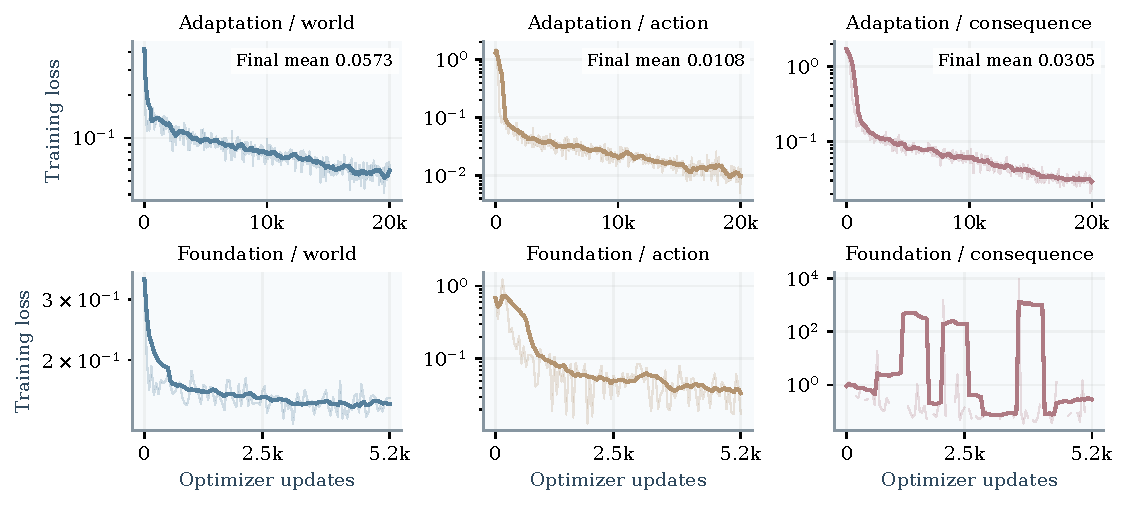
\includegraphics[width=\linewidth]{Figures/training.pdf}
\caption{\textbf{How do the joint objectives optimize?} Measured foundation training (top) and completed LIBERO adaptation (bottom). Thin traces retain logged batches and outliers; thick traces average up to 11 records with available supervision. Each objective uses a logarithmic scale. The dotted boundary marks the concurrent mixture, label-mask, and sharding changes at update 8,400; smoothing starts anew there.}
\label{fig:training}
\end{figure}

\subsection{Experimental setup and evaluation}
\label{app:setup}
\textbf{Data and splits.}
Table~\ref{tab:corpus} distinguishes data consumed by the archived run from prepared and acquired
expansions. The first mixture samples DROID, Bridge, and EgoDex with probabilities 50.88\%, 20.43\%,
and 28.69\%. The five-source stage uses temperature 0.7 on training-window counts and probabilities
40.44\%, 16.24\%, 22.80\%, 4.66\%, and 15.87\% in table order. The cache reserves an episode-level
holdout using a deterministic one-in-ten partition. All windows from an episode follow that
partition. Ego4D instead groups clips by source video: its merged cache contains 436,116 training
and 50,856 holdout windows from 592 and 72 video identifiers, with zero shared identifiers.
The first Ego4D cache supplies world supervision; consequence supervision requires an admitted
tracking pipeline. Dataset availability and exposure during optimization are recorded separately.

\begin{table}[H]
\centering\small
\begin{tabularx}{\linewidth}{@{}lCCC@{}}
\toprule
Source & Stage & Targets & Train windows \\
\midrule
\panelrow{4}{A. Consumed after the 8,400-update resume}
DROID & Active & World, action & 1,674,648 \\
BridgeData V2 & Active & World, action & 454,690 \\
EgoDex & Active & World, consequence & 738,550 \\
RoboMIND Franka & Active & World, action & 76,446 \\
RoboMIND UR5e & Active & World, action & 439,974 \\
\midrule
\panelrow{4}{B. Next admissions; outside the consumed mixture}
Ego4D & Merged & World & 436,116 \\
RoboMIND AgileX & Encoding & World, action & Pending \\
InternData-A1 & Acquiring & World, action & Pending \\
RoboCOIN subset & Encoding & World, action & Pending \\
EPIC-KITCHENS-100 & Acquiring & World & Pending \\
\bottomrule
\end{tabularx}
\caption{\textbf{Pretraining inventory at the evidence snapshot.} Counts are cached training windows, not unique trajectories or duration. Targets describe the admitted or intended adapter. The expansion rows carry no sampling probability until training admission.}
\label{tab:corpus}
\end{table}

RoboMIND AgileX supplies the next bimanual data source. Its inspected export covers 10,269 episodes,
with encoding still in progress. InternData-A1 acquisition spans multiple embodiments; the first
RoboCOIN tranche contains 38 selected corpus repositories. Additional Ego4D access and an
AgiBotWorld-Beta subset remain conditional on access and validation. The current selection omits
RT-1, CALVIN, RoboSet, and RH20T. LIBERO, RoboTwin2.0-Full, VLABench, RoboCasa365 target tasks,
and RoboDojo are reserved for downstream training. LIBERO-Plus and LIBERO-PRO supply evaluation
only. Future corpus revisions must preserve these evaluation boundaries.

\textbf{Model and optimization.}
The world stream uses Wan2.2-TI2V-5B through its released Diffusers implementation, initialized with
public video weights. The agent stream is trained from scratch. The combined model has approximately
6.02 billion parameters, including a 1.02-billion-parameter agent with width 1,024 and 30 layers.
Both streams use 24 attention heads of dimension 128. The video autoencoder and text encoder remain
frozen. Foundation training uses eight H200 accelerators, a batch of 16 per device, and four
accumulation steps, giving a global batch of 512. AdamW uses world/agent learning rates of
0.00005/0.0001, momentum coefficients 0.9/0.95, weight decay 0.01, and gradient clipping at 1. The
planned budget is 60,000 updates with 1,500 warmup updates and a final 6,000-update decay. All three
loss weights are 1. The resolved configuration uses independent corruption levels and zero explicit
boundary-sampling probability. The completed direct-adaptation run uses four H200 accelerators,
global batch 64, and a cosine learning-rate schedule; Appendix~\ref{app:details} records the remaining adaptation settings.

\textbf{Tasks and comparison protocol.}
The core downstream arenas are LIBERO \citep{libero}, RoboTwin 2.0 Full \citep{robotwin}, VLABench
\citep{vlabench}, and the RoboCasa365 target-task split \citep{robocasa365}, with RoboDojo supplying additional
capability tests. Direct adaptation
starts from the public video initialization plus a fresh agent; pretrained adaptation starts from a
JAM foundation release. The paired comparison fixes the demonstrations, action adapter, training
budget, sampler, and environment version. LIBERO-Plus \citep{liberoplus} and LIBERO-PRO
\citep{liberopro} supply robustness tests. RoboTwin clean-to-randomized transfer is evaluated
separately from training on its Full mixture. The proposed final protocol uses three training seeds,
50 trials per LIBERO task, and the official one-trial-per-variant LIBERO-Plus enumeration. Each
remaining suite follows its pinned task and reset manifest. Full-suite external averages remain
distinct from the current task-subset experiments.

\textbf{Metrics and statistics.}
Control is measured by task success rate, with subtask progress retained where supplied by the
benchmark. World prediction uses perceptual image distance and tracked-motion error. Consequence
prediction uses average displacement error in image-normalized coordinates and visibility
calibration. Frozen-world probes predict actions and consequences from intermediate world features
with generated action and consequence inputs fully corrupted. A shuffled-label probe and an
observation-only predictor establish reference levels. Planned uncertainty estimates use a paired
hierarchical bootstrap over training seeds, tasks, and shared episode resets with 10,000 resamples
and 95\% intervals. Final open-loop comparisons use episode-level resampling. The preliminary probes below use
window-level sampling and their separately stated bootstrap protocol.


\subsection{Controls required by the scientific question}
\label{app:controls}
\textbf{Separating information and gradients.}
World-only pretraining supervises future video. Action-only pretraining supervises commands.
Independent multitask pretraining supervises both with separate generated-stream computations.
Auxiliary supervision reads detached world features. The attached one-way arm uses the same
visibility while allowing action gradients through world keys and values. Reciprocal JAM
additionally exposes agent keys and values to world queries. Each pretraining arm receives the same
source sequence and then the same downstream adaptation procedure. Direct adaptation from public
video weights supplies the separate baseline for the value of embodied pretraining.

Strict isolation of coupling requires identical clean conditions in every arm. In the audited
implementation, disabling agent visibility also removes the state token from the world stream's
attention. The existing visibility switches therefore change both generated-token exchange and part
of the conditioning interface. The planned comparison routes equivalent static state and
current-observation information to every arm before interpreting a performance difference as an
effect of coupling. The paper's target table describes this stricter protocol, whose results remain
awaiting measurement. It does not treat the existing switches as an already completed controlled
experiment.

\textbf{Representation probes and interventions.}
The measured milestone study freezes the world parameters and reads frame-mean features at layers
5, 10, 15, 20, 25, and 29. Initial observations remain clean; future-world inputs use corruption
level 0.5. Action and consequence inputs are pure Gaussian noise. Each source contributes up to
4,000 windows from its held-out corpus partition, split into 2,800 probe-training and 1,200
probe-test windows. These internal splits operate on windows and can share episodes. Ridge
regularization is selected on a quarter of the probe-training windows and the final readout is
refitted on that training split. The grid spans 1 through 100,000. Action R-squared intervals use
1,000 bootstrap resamples over test windows. Figure~\ref{fig:representation} reports every sampled
layer for JAM, the video prior, and a randomly initialized world stream. Copy-first and shuffled-label
controls accompany the archived reports. Consequence displacement above magnitude 8 is masked.

This diagnostic tests readout from partially observed future dynamics. Establishing a pretraining
effect under matched coupling controls additionally requires episode-disjoint probe fitting,
observation-only controls, and matched information at extraction. A capacity-matched nonlinear
readout can then separate information accessibility from probe capacity. The current probe scores
are preliminary representation measurements with the stated visible future context.

Action shuffling tests sensitivity to the action input. Counterfactual prediction additionally
requires a target future obtained by executing the alternative action from the same simulator state.
The intervention protocol therefore saves a reset state, executes each admissible command sequence,
and scores each generated future against its matching rollout. Corruption tests vary timing and
command magnitude within valid control limits. This distinguishes sensitivity from correct
prediction of an intervention.

Consequence conditioning compares commands alone, observed consequences alone, and both together on
the same test windows. Predicted consequences form a separate condition that retains their model
error. The resulting gap measures the cost of prediction and any distribution shift at the
conditioning interface. A held-out-embodiment study excludes the target platform from pretraining
and fixes its downstream demonstration budget. Camera configuration, temporal duration, and
available keypoint groups accompany each result.

\textbf{Conditional sampling checks.}
Every conditional use specifies all generated variables. An action-clamped world sampler must
continue integrating unobserved consequences. The updated sampler implements that independent
consequence schedule, correcting the earlier coupling to the clamped action level. The archived
post-correction test uses the update-5,100 checkpoint, 300 LIBERO holdout windows, and 10 Euler steps.
Donor, hold, and time-shuffled actions produce small consequence-error changes whose paired
95\% intervals all include zero. Figure~\ref{fig:representation} uses this corrected report. It
measures action-input sensitivity against the observed future, while counterfactual fidelity
requires the separately executed futures described above. Conditional benchmark evaluation remains
pending. Independent corruption levels define a training family; each deployment path also requires
a fidelity check.

\FloatBarrier

\subsection{Evidence boundaries and failure analysis}
\label{app:evidence}
The evidence package contains the completed adaptation log, its result summary, a fixed prefix of
the ongoing foundation log, and sanitized resolved configurations. The public manifest records
source paths, file hashes, the audit revision, and the status of each artifact. Local asset paths
are replaced by logical references in the published configurations; original-file hashes preserve
the connection to the inspected source. These configuration snapshots document the runs and are not
standalone launch configurations.

The LIBERO closed-loop evaluation was interrupted before a complete suite result file was produced.
Partial rollout videos therefore contribute neither success rates nor selected qualitative evidence
to the paper. Foundation transfer and coupling ablations await completed runs. The milestone probes and
post-correction sensitivity report are measured diagnostics with the limitations stated above.
External reference results retain their own provenance and evaluation scope. The planned tables and
scaling figure use design values inherited or extended from the working manuscript; they are layout
targets rather than preregistered outcomes or model predictions.

The data audit identified extreme displacement labels in some human-video windows. A displacement
mask rejects magnitudes above 8 from the 8,400-update resume onward. The same resume changes the
source mixture, maps absent modalities to pure-noise inputs, and changes the sharding topology.
The first segment retains the original label distribution. Figure~\ref{fig:training} preserves this
boundary and its raw losses. Attributing a change to the label filter requires a matched comparison.
Camera motion, occlusion, and the gap between observed and predicted consequences remain additional
failure settings.

\subsection{External reference results}
\label{app:reference}
Each main benchmark has a dedicated table with all baseline rows present in its source export.
Table~\ref{tab:libero} supplies the standard LIBERO suites alongside the robustness tables in the
main text. R1 is the external method identified by the immutable source link, distinct from JAM.
The website aggregates source-reported evaluations; its presence alone does not establish that
all baseline runs share one evaluation implementation. The archive retains original numeric strings,
model labels, source revisions, and a cell-level rendering map. The official export contains no
LIBERO-PRO table, so Table~\ref{tab:libero_pro} uses the benchmark maintainers' own leaderboard.
Its normalized values are multiplied by 100 exactly. Its reported totals are preserved despite
model-dependent coverage of environment tests. External protocol scopes remain attached to their
values until a matched JAM evaluation is available.
\begin{table}[H]
\centering
\begingroup\fontsize{9.2}{10.5}\selectfont
\setlength{\tabcolsep}{2.5pt}\renewcommand{\arraystretch}{1.08}
\begin{tabularx}{\linewidth}{@{}p{1.43in}CCCCC@{}}
\toprule
\panelrow{6}{LIBERO}
Model & Spatial & Object & Goal & Long & Mean \\
\midrule
OpenVLA & 84.7 & 88.4 & 79.2 & 53.7 & 76.5 \\
$\pi_0$ & 98.0 & 96.8 & 94.4 & 88.4 & 94.4 \\
StarVLA & 97.8 & 98.6 & 96.2 & 93.8 & 96.6 \\
$\pi_{0.5}$ & 98.8 & 98.2 & 98.0 & 92.4 & 96.9 \\
GR00T-N1.6 & 97.7 & 98.5 & 97.5 & 94.4 & 97.0 \\
OpenVLA-OFT & 97.6 & 98.4 & 97.9 & 94.5 & 97.1 \\
X-VLA & 98.2 & 98.6 & 97.8 & 97.6 & 98.1 \\
ABot-M0 & 98.8 & 99.8 & 99.0 & 96.6 & 98.6 \\
Being-H0.5 & 99.2 & 99.6 & 99.4 & 97.4 & 98.9 \\
Qwen-RobotManip & \nr & \nr & \nr & \nr & 99.2 \\
\midrule
Fast-WAM & 98.2 & \textbf{100.0} & 97.0 & 95.2 & 97.6 \\
Motus & 96.8 & 99.8 & 96.6 & 97.6 & 97.7 \\
ImageWAM & 97.2 & 99.2 & 98.8 & 98.4 & 98.4 \\
LingBot-VA & 98.5 & 99.6 & 97.2 & \textbf{98.5} & 98.5 \\
DiT4DiT & \nr & \nr & \nr & \nr & 98.6 \\
Being-H0.7 & \nr & \nr & \nr & \nr & 99.2 \\
ABot-M0.5 & \textbf{100.0} & 99.8 & 99.4 & 98.4 & \textbf{99.4} \\
R1 & 99.6 & 99.6 & \textbf{99.8} & 98.2 & 99.3 \\
\midrule
\jamshade\textbf{JAM} & \multicolumn{5}{c}{\pendingresult} \\
\bottomrule
\end{tabularx}
\endgroup
\caption{\textbf{LIBERO task success.} The four suites measure spatial, object, goal, and long-horizon control. Source: \refsource{}. \benchmarknote}
\label{tab:libero}
\end{table}

\FloatBarrier

\subsection{Reproduction and experiment ledger}
Measured logs, external references, and layout targets occupy separate artifact files. The README gives the complete build procedure. The commands \texttt{python3} \path{scripts/build_artifacts.py} and \texttt{python3} \path{scripts/validate.py} regenerate the numerical displays and check evidence consistency, respectively.

The protocol ledger links each scientific question to inspected source configurations and required
result artifacts. It identifies controls that still require implementation changes. Promoting a
target to a measurement requires its result file, checkpoint, evaluation manifest, and aggregation
command; the corresponding scientific claim is then reviewed against that evidence.
